\documentclass[unknownkeysallowed,usepdftitle=false]{beamer}
% unknownkeysallowed is needed for mac and the newer latex version -> is more picky than before...
\usetheme[headheight=1cm,footheight=2cm]{boxes}
%\usetheme{default}

\usepackage{inputenc}
\usepackage{default}
\usepackage{graphicx}
\usepackage{epsfig}
\usepackage{siunitx}
\usepackage{color}
\usepackage{ifthen}
\usepackage{ragged2e}

\setbeamertemplate{navigation symbols}{}%remove navigation symbols
\setbeamersize{text margin left=0pt,text margin right=0pt} % text and figures flush to edges

% some colors
\definecolor{grau}{gray}{.5}
\definecolor{slfcolor}{rgb}{0,0.5,0.8353}
\definecolor{wslcolor}{rgb}{0,0.4,0.4}

% setup links
\hypersetup{%
	%linkbordercolor=green,%
	colorlinks=false,%
	pdfborderstyle={/S/U/W 0},%
	%pdfpagemode=FullScreen,%
	pdfstartpage=4%
	}

% setup some fonts
\setbeamerfont{title}{series=\bfseries, size=\small}
\setbeamerfont{author}{size*={5pt}{0pt}}
\setbeamerfont{institute}{size*={3pt}{0pt}}
\setbeamerfont{bodytext}{size=\scriptsize}


% Title setup	
\title{Absolute Velocity Estimates from a Glider Mounted ADCP}
\author{Callum Rollo\inst{1} (\texttt{c.rollo@uea.ac.uk}) \and Karen J Heywood\inst{1} \and Rob Hall\inst{1} \and Alex Phillips\inst{2}}
\institute{\inst{1}University of East Anglia, Norwich, UK
\quad \inst{2}Marine Autonomous Robotics Systems group, Southampton UK}
% add title in headbox
\setbeamertemplate{headline}
{\leavevmode
\begin{beamercolorbox}[width=1\paperwidth]{head title}
  % LOGO
  \begin{columns}[t, totalwidth=\textwidth]
  \begin{column}[c]{1.05cm}
     
\includegraphics[height=1.05cm]{figure/graphic_egu_photo_yes.png}
  \end{column}
  % TITLE
   \begin{column}[c]{10.6cm}
   \centering \usebeamerfont{title} \textcolor{slfcolor}{\inserttitle} \\
   \centering \usebeamerfont{author} \color[rgb]{0,0,0} \insertauthor \\
   \vspace{-0.05cm}
   \centering \usebeamerfont{institute} \insertinstitute
  \end{column}
  % PICUTRE
  \begin{column}[c]{1.0cm}
    \hspace{0.005cm}
    
\includegraphics[trim=100 100 100 500,clip,height=1.05cm]{figure/face.jpg}
  \end{column}
  \end{columns}
  {\color{slfcolor}\hrule height 1pt\vspace{0.1cm}}
\end{beamercolorbox}%
}

% setup the navigation in footbox
% first set some button colors
\newcommand{\buttonactive}{\setbeamercolor{button}{bg=wslcolor,fg=white}}
\newcommand{\buttonpassive}{\setbeamercolor{button}{bg=slfcolor,fg=white}}
% now set up that the one active one gets the new color.
\newcommand{\secvariable}{nothing}
% therefore we write before each section (well, everything which should be part of the navi bar)
% the variable \secvariable to any name which is in the next function ...
\newcommand{\mysection}[1]{\renewcommand{\secvariable}{#1}
}
% ... compaired to strings in the following navibar definition ...
\newcommand{\tocbuttoncolor}[1]{%
 \ifthenelse{\equal{\secvariable}{#1}}{%
    \buttonactive}{%
    \buttonpassive}
 }
% ... here we start to set up the navibar. each entry is calling first the function \tocbuttoncolor with the argument which should be tested for being active. if active, then change color. afterwards the button is draw. so to change that, you need to change the argument in \toc..color, the first in \hyperlink and before each frames definition... A bit messed up, but works...
\newlength{\buttonspacingfootline}
\setlength{\buttonspacingfootline}{-0.2cm}
\setbeamertemplate{footline}
{\leavevmode
\begin{beamercolorbox}[width=1\paperwidth]{head title}
  {\color{slfcolor}\hrule height 1pt}
  \vspace{0.05cm}
  % set up the buttons in an mbox
  \centering \mbox{
    \tocbuttoncolor{intro}
    \hyperlink{intro}{\beamerbutton{Introduction}}
    \tocbuttoncolor{trial_shear}
    \hspace{\buttonspacingfootline}
      \hyperlink{trial_shear}{\beamerbutton{Oban shear}}
    \tocbuttoncolor{line}
    \hspace{\buttonspacingfootline}
      \hyperlink{line}{\beamerbutton{Line Features}}
    \tocbuttoncolor{major}
    \hspace{\buttonspacingfootline}
      \hyperlink{major}{\beamerbutton{Major Surges}}
    \tocbuttoncolor{slab}
    \hspace{\buttonspacingfootline}
      \hyperlink{slab}{\beamerbutton{Slab Release}}
    \tocbuttoncolor{minor}
    \hspace{\buttonspacingfootline}
      \hyperlink{minor}{\beamerbutton{Minor Surges}}
    \tocbuttoncolor{friction}
    \hspace{\buttonspacingfootline}
      \hyperlink{friction}{\beamerbutton{Friction}}
    \tocbuttoncolor{conclusion}
    \hspace{\buttonspacingfootline}
      \hyperlink{conclusion}{\beamerbutton{Conclusion}}
    % this last one should normaly not be used... it will open the preferences to change the 
    % behaviour of the acrobat reader in fullscreen -> usefull in pico...
    \setbeamercolor{button}{bg=white,fg=black}
    % for presentation
    %\hspace{-0.1cm}\Acrobatmenu{FullScreenPrefs}{\beamerbutton{\#}}
    % for upload
    
     
\Acrobatmenu{FullScreenPrefs}{\vspace{0.3cm}\hspace{0.24cm}\mbox{%
      \includegraphics[height=0.04\textheight,keepaspectratio]{%
	  figure/CreativeCommons_Attribution_License}%
	  }}
   }
    \vspace{0.05cm}
\end{beamercolorbox}%
}



\begin{document}


%%%%%%%%%%%%%%%%%%%%%%%%%%%%%%%%%%%%%%%%%%%%%%%%%%%%%%%%%%%%%%%%%%%%%%%%%%
\mysection{intro}
%%%%%%%%%%%%%%%%%%%%%%%%%%%%%%%%%%%%%%%%%%%%%%%%%%%%%%%%%%%%%%%%%%%%%%%%%%
\begin{frame}\label{\secvariable}
\usebeamerfont{bodytext}
\justifying

\vspace*{-1.2mm}    
%\hspace*{-\beamerleftmargin}
%\hspace*{-1.05cm}
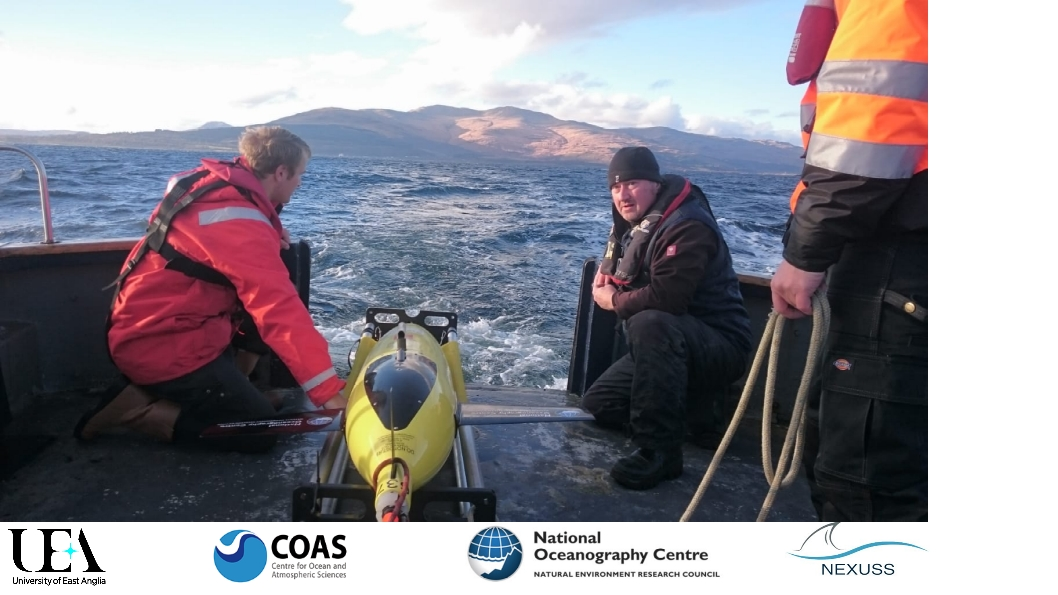
\includegraphics[trim=0 0 100 5,clip,width=\paperwidth]{figure/splash.jpg}

%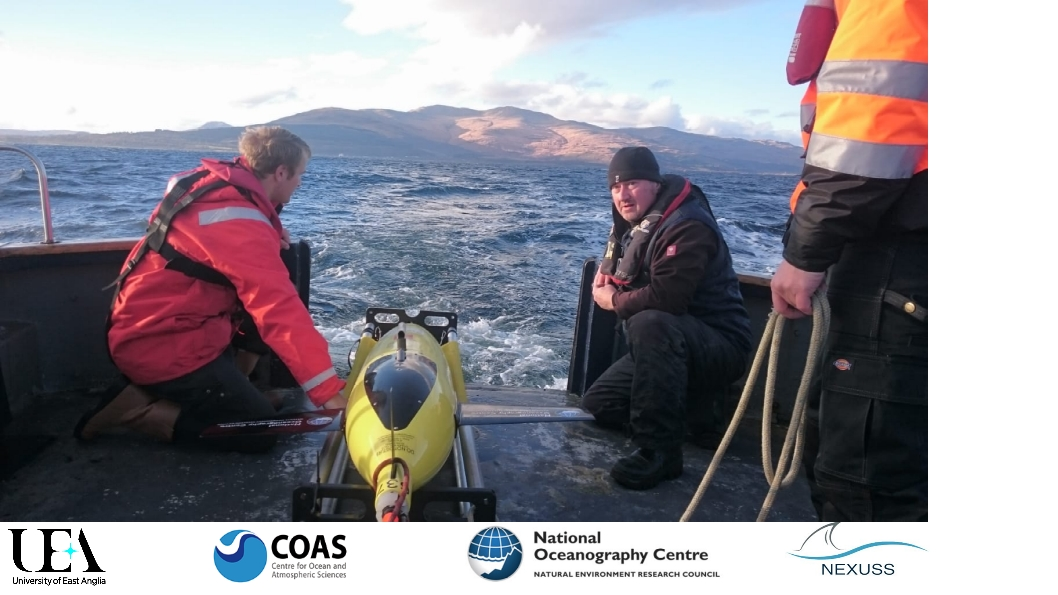
\includegraphics[trim=0 0 0 0,clip,width=1.2\textwidth,keepaspectratio]{figure/splash.jpg}\\


\end{frame}

%%%%%%%%%%%%%%%%%%%%%%%%%%%%%%%%%%%%%%%%%%%%%%%%%%%%%%%%%%%%%%%%%%%%%%%%%%
\mysection{trial_shear}
%%%%%%%%%%%%%%%%%%%%%%%%%%%%%%%%%%%%%%%%%%%%%%%%%%%%%%%%%%%%%%%%%%%%%%%%%%
\begin{frame}\label{\secvariable}
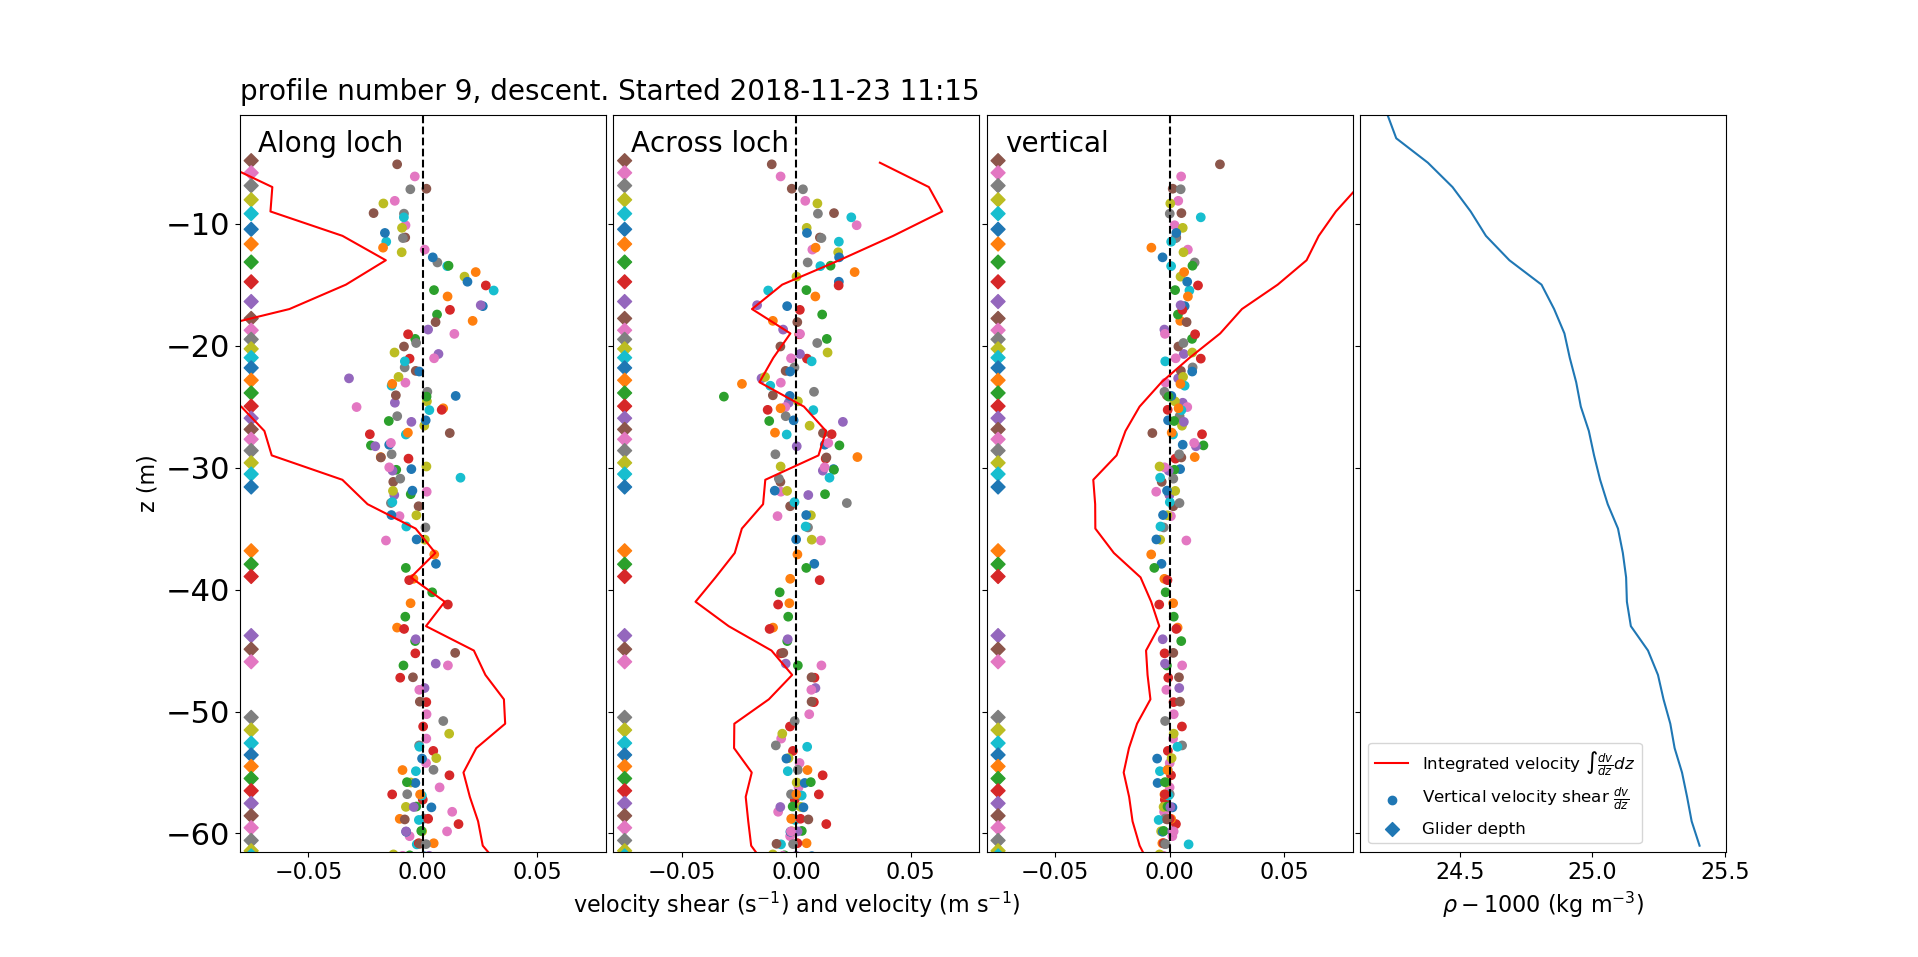
\includegraphics[trim=70 20 80 80,clip,width=\paperwidth]{figure/95_qc.png}

\begin{itemize}
\item Vertical shear of horizontal velocity coherent between ensembles
\item Strong along loch shear across pycnocline
\end{itemize}
  
\end{frame}

%%%%%%%%%%%%%%%%%%%%%%%%%%%%%%%%%%%%%%%%%%%%%%%%%%%%%%%%%%%%%%%%%%%%%%%%%%
\mysection{line}
%%%%%%%%%%%%%%%%%%%%%%%%%%%%%%%%%%%%%%%%%%%%%%%%%%%%%%%%%%%%%%%%%%%%%%%%%%
\begin{frame}\label{\secvariable}
\begin{center}
  \vspace{-0.5cm}
 
\includegraphics[width=1\textwidth,height=0.8\textheight,keepaspectratio]{%
  figure/PIC1.jpg}
\end{center}
  \vspace{-0.5cm}
  \textbf{a)} GEODAR show many approaching line features\\
  \textbf{b)} Flow-height measured by upward--looking FMCW radar.\\
  $\quad \Rightarrow$ Line features correspond to waves: We call them surges.
  
\end{frame}

%%%%%%%%%%%%%%%%%%%%%%%%%%%%%%%%%%%%%%%%%%%%%%%%%%%%%%%%%%%%%%%%%%%%%%%%%%
\mysection{major}
%%%%%%%%%%%%%%%%%%%%%%%%%%%%%%%%%%%%%%%%%%%%%%%%%%%%%%%%%%%%%%%%%%%%%%%%%%
\begin{frame}\label{\secvariable} %%Eine Folie
\begin{center}

\includegraphics[width=1\textwidth,height=0.8\textheight,keepaspectratio]{%
figure/PIC1.jpg}
\end{center}
\begin{columns}
\begin{column}[t]{1.1\textwidth}
 Major surges can exist in the avalanche body and they overrun each other.\\
 The origin of the major surges are secondary slab release (colored bars).
\end{column}
\end{columns}
\end{frame}

%%%%%%%%%%%%%%%%%%%%%%%%%%%%%%%%%%%%%%%%%%%%%%%%%%%%%%%%%%%%%%%%%%%%%%%%%%
\mysection{slab}
%%%%%%%%%%%%%%%%%%%%%%%%%%%%%%%%%%%%%%%%%%%%%%%%%%%%%%%%%%%%%%%%%%%%%%%%%%
\begin{frame}\label{\secvariable}

\includegraphics[width=1\textwidth,height=0.8\textheight,keepaspectratio]{%
figure/PIC1.jpg}
\begin{columns}
\begin{column}[t]{1.1\textwidth}
 Video and laserscan data reveal the occurrence of slab releases.\\
 Around \SI{50}{\percent} of the total entrained volume entered the flow via
slabs.\\
  The slabs can be as large as the initial released slab.
\hyperlink{slabtable}{\beamerbutton{more \dots}}
\end{column}
\end{columns}
\end{frame}



\begin{frame}\label{slabtable}
\begin{columns}
\begin{column}[t]{1.1\textwidth}
\hyperlink{slab}{\beamerbutton{\dots back to figure}}\\
Slabs enter at random locations into the flowing avalanche and their mass is not
concentrated at the front.\\
$\quad \Rightarrow$ Spreading the mass over the flow alters the runout.
\vspace{0.3cm}
\end{column}
\end{columns}
\usebeamerfont{bodytext}
 \begin{tabular}{c|rr@{}c@{}rrrrr}
 \setlength{\tabcolsep}{6mm}
   & Time & \multicolumn{3}{r}{Volume} & Range & Length & Area & Depth \\
   & [\si{\second}] & \multicolumn{3}{r}{[\si{\cubic\metre}]} & [\si{\metre}] &
[\si{\metre}] & [\si{\square\metre}] & [\si{\metre}]\\\hline

   \textbf{Avalanche~\#0019} & & $V_t$ &=& 29500 & & & 40411 & 0.73 \\
   initial release &3.4& $V_0$ &=& 2188 & 2506 &  62 &  1400 & 1.56 \\
   slab \#1 & 17.2    &  $V_1$ &=&  521 & 2356 &  39 &   701 & 0.74 \\
   slab \#2 & 23.4    &  $V_2$ &=& 3503 & 2284 &  83 &  2753 & 1.28 \\
   slab \#3 & 20--25$^*$ &  $V_3$ &=& 3345 & 2150 &  99 &  1880 & 1.78 \\
   slab \#4 & 38.7    &  $V_4$ &=& 4276 & 1945 & 153 &  3657 & 1.17 \\
   \\
   \textbf{Avalanche~\#0017} & &  $V_t$ &=& 78500 & & & 82632 & 0.95\\
   initial release&5.2&  $V_0$ &=& 15233 & 2402 & 191 & 12974 & 1.17\\
   slab \#5 & 12.2    &  $V_5$ &=&  7620 & 2219 & 202 &  6043 & 1.26 \\
   slab \#6 & 14.1    &  $V_6$ &=&  5868 & 2215 & 166 &  5851 & 1.01 \\
   slab \#7 & 25.6    &  $V_7$ &=&  6307 & 1982 &  95 &  3320 & 1.90 \\
   slab \#8 & 15--25$^*$ &  $V_8$ &=& 10663 & 1947 & 253 &  5037 & 2.12
 \end{tabular}
 
\vspace{0.2cm}
 \textbf{Table:} Release time, Volume, Location and size parameters of all
identified slabs.

\end{frame}




%%%%%%%%%%%%%%%%%%%%%%%%%%%%%%%%%%%%%%%%%%%%%%%%%%%%%%%%%%%%%%%%%%%%%%%%%%
\mysection{minor}
%%%%%%%%%%%%%%%%%%%%%%%%%%%%%%%%%%%%%%%%%%%%%%%%%%%%%%%%%%%%%%%%%%%%%%%%%%
\begin{frame}\label{\secvariable} %%Eine Folie
\begin{center}

\includegraphics[width=1\textwidth,height=0.7\textheight,keepaspectratio]{%
figure/PIC1.jpg}
\end{center}
\vspace{-0.2cm}
\begin{columns}
\begin{column}[t]{1.1\textwidth}
Minor surges are only found in the head of large powder avalanches.\\
They are flow features (roll waves) in the energetic
frontal region.\\
Their speed is high and constant when behind the front, but dramatically \\
$\quad$ decelerate as soon they overtake the leading edge.

\end{column}
\end{columns}

\end{frame}

%%%%%%%%%%%%%%%%%%%%%%%%%%%%%%%%%%%%%%%%%%%%%%%%%%%%%%%%%%%%%%%%%%%%%%%%%%
\mysection{friction}
%%%%%%%%%%%%%%%%%%%%%%%%%%%%%%%%%%%%%%%%%%%%%%%%%%%%%%%%%%%%%%%%%%%%%%%%%%
\begin{frame}\label{\secvariable}
\hspace{-0.6cm}

\includegraphics[width=0.6\textwidth,height=0.7\textheight,keepaspectratio]{%
figure/PIC1.jpg}

\includegraphics[width=1\textwidth,height=0.46\textheight,keepaspectratio]{%
figure/PIC1.jpg}

\begin{columns}
\begin{column}[t]{1.1\textwidth}
Minor surges were simulated with a 1D Voellmy--like model.\\
Model \#1 describes the front, thats what usual models do.\\
Model \#2 tries to follow every surge individually, but no deceleration.\\
Model \#3 explains minor surges with 2 sets of friction
parameters\\
\vspace{0.2cm}
$\Rightarrow$ The effective friction changes dramatically as soon as\\
\raggedleft the surge reaches the front\\
\raggedright $\Rightarrow$ The avalanche body experiences different flow
conditions as the front.
\end{column}
\end{columns}

\end{frame}

%%%%%%%%%%%%%%%%%%%%%%%%%%%%%%%%%%%%%%%%%%%%%%%%%%%%%%%%%%%%%%%%%%%%%%%%%%
\mysection{conclusion}
%%%%%%%%%%%%%%%%%%%%%%%%%%%%%%%%%%%%%%%%%%%%%%%%%%%%%%%%%%%%%%%%%%%%%%%%%%
\begin{frame}\label{\secvariable}
  
  \begin{itemize}
   \item GEODAR radar is able to track internal surges (flow height waves)
below the powder cloud of snow avalanches.
   Two types of surges exist: \textit{Major} and \textit{Minor surges} are
differentiated by their length.
  \item Major surges can occur at random location in the flow and influence the
mass distribution of the avalanche.
   Minor surges are ubiquitous feature of the fast--flowing energetic
part in the frontal region of large powder avalanches. 
  \item The effective friction between the front and the avalanche body
differs. This must be explained with changes in the snow surface like smoothing
and entrainment of the soft, upper snow layers. Numerical models not yet account for this.

  \end{itemize}

  \usebeamerfont{bodytext}
Original template by Anselm K\"ohler\\ \texttt{https://github.com/snowtechblog/pico-latex-presentation}

\end{frame}



\end{document}
